\newpage
\chapter{Implementation}

This chapter is about how to implement the requirements using the knowledges that has been described in the \textit{Methodology} chapter.

\section{Programming}

This section will describe the programming fundamental, infrastructure and also superstructure of the implementation. 

A project named \textbf{LoYiW} (\textit{Locate Yourself in WLAN}) has been created to implement the functions. The programming requirements are: \textit{client GUI} and \textit{administration GUI}. As explained before, the client GUI must be implemented using B/S(\textit{browser/server}) structure, but the administration GUI could be implemented using either B/S or C/S(\textit{client/server}) structure. 

So the programming language must be able to generate a website. If the administration GUI prefer to use the C/S structure, the programming language must be able to generate a desktop GUI. Even though it is not necessary, that the client and administration GUI use the same technology, it is properly to use the same programming language, which may reduce the complexity of the \textit{LoYiW} project, it may also reduce the software maintenance cost in the future.

There are plenty programming languages that are able to fulfil the requirements, almost all the popular programming languages, like C++, PHP, Java, Ruby, C\#.NET, Python, could solve it. The \textit{LoYiW} project chooses Python, but it does not mean that Python is the only available language.

First, will describe the programming fundamental knowledge.

\subsection{Python}

\textbf{Python}\footnote{Python official website: \url{http://www.python.org/}} is an interpreted, object-oriented, high level scripting and programming language. It was first introduced in 1991 by Guido van Rossum, who wanted to develop a language that could be used for anyone. The syntax of Python is simple and clear, one of the features is white space as a statement indentation. When Python program is executed, first .py file in the source code is compiled into byte code, and then it performs this compiled byte code by the Python Virtual Machine. This mechanism is the same with Java and .NET.  

Python has two popular versions: Python 2 and Python 3, their concurrent versions are Python 2.7 and Python 3.5. A lot of features has been changed from Python 2 to Python 3. Because of the limitation of Kivy (See next section), Python 2 is used as the main programming language of this project.

As a famous script language, Python has a lot of advantages:

\begin{itemize}
	\item Python is free, open source, ease of learning, portability, dynamic typing and integration with other languages.
	\item Python is written by C language, a lot of standard libraries and other libraries are written also in C, so it runs very fast.
	\item Python source code is generally considered to have better readability, and it supports large-scale software development.
	\item It is a multi-paradigm programming language, used to code in several different programming styles. A programmer can code in a functional, object oriented or imperative format.
	\item Python can be run in interactive mode, such as on operating system Unix / Linux, OS X or Windows which have native support of Python interactive environment by command mode.
\end{itemize}

However, in Python several disadvantages still exist: 

\begin{itemize}
	\item Unique syntax, the most common situation is that mixed tab and space cause an error, but this is difficult to distinguish. 
	\item Python is an interpreted language at runtime, it adds the overhead on interpretation to the runtime of the program which can lead to a slower (means then Java or C/C++.) runtime.  
	\item Language translation,  it is not very simple to translate a Python program into any other language. The translation from Python to another language would require the user to carefully examine the structure of the code.
\end{itemize}

\subsubsection{Python modules}

A Python module allows a programmer to logically organize the Python code. Grouping related code into a module makes the code easier to understand and to use. In a nut shell, a Python module is a file consisting of Python code, it can define functions, classes and variables, and can also include runnable code.

Python module is also called \textit{library} in other programming language. Several Python modules have been used in \textit{LoYiW} project, they are listed below.

\subsection{Kivy}
\textbf{Kivy}\footnote{Kivy official website: \url{http://kivy.org/}} is an open source and free Python framework, used for rapid development of mobile applications or other multi-touch applications. It's distributed under the MIT license.

Kivy has been elected as the GUI framework in this master thesis, but Kivy supports only Python 2 for now on, so the GUI are programmed with Python 2.

\subsubsection{Advantages of Kivy}
Kivy has the following advantages:

\begin{itemize}
	\item open source and free.
	\item Multi-platform: Just one set of code can be run on the desktop or mobile platforms and it supports most original input protocols and equipment.
	\item extensive API documentation and development Guide.
\end{itemize}

\subsubsection{KV language}
The \textbf{KV language} (sometimes called \textit{kvlang}, or \textit{kivy language}), used for the creation of widget tree in a declarative way and to bind widget properties to each other or to callbacks in a human natural manner. It allows for very fast prototyping and agile changes to the GUI. It also facilitates a good separation between the logic of your application and its User Interface.

\subsection{JSON}
\textbf{JSON} means \textit{JavaScript Object Notation}, is a lightweight and human readable data interchange format. It is based on a subset of \textit{JavaScript}. JSON is a pure text format that is completely language- and plattform independent.

The \textit{LoYiW} project uses JSON as the configuration file format. The configuration files are stored in \textit{configs} folder.

\subsection{Shell script}

A Unix shell is a command language interpreter. \textbf{Shell script}, or \textit{shell command language}, is a programming language defined in the POSIX standard\footnote{Definition of \textit{Shell Command Language}: \url{http://pubs.opengroup.org/onlinepubs/009695399/utilities/xcu_chap02.html}}. \textit{Bash} could be considered as an implementation of \textit{shell}\footnote{BashScripting(Deutsch): \url{https://help.ubuntu.com/community/Beginners/BashScripting}}.

The operating system OS X Macintosh supports also \textit{shell}, because it is also an Unix-like operating system.

There are several command-line tasks that should be executed in a row, so \textit{shell script} is the best choice to do so.

The \textit{shell script} in the \textit{LoYiW} project is written in \textit{LoYiW/shells/mac.sh}, it contains two functions: start/stop redirection and start/stop server. Before running of the \textit{mac.sh}, the \textbf{su}(\textit{super user}) password, the port number, and the IP address of the web server (which is the \textit{redirection target} also) should be configured at the beginning of the \textit{mac.sh} at first.

\begin{lstlisting}[language=bash, caption={Configurations sample in mac.sh}]
PASSWORD='password' # Super user password
PORT=80 # Defualt HTTP port number
TARGET_IP=192.168.2.1 # IP address of the web server
\end{lstlisting} 

This shell script file could be executed on Macintosh computer (Tested on OS X 10.11 El Capitan):

\begin{lstlisting}[caption={Start/stop redirection/server sample}]
# Start the redirection
shells/mac.sh redirect=start

# Stop the redirection
shells/mac.sh redirect=stop

# Start the web server
shells/mac.sh server=start

# Stop the web server
shells/mac.sh server=stop
\end{lstlisting}

\begin{lstlisting}[language=bash, caption={Redirection is implemented using also shell script, see shells/mac.sh for more details.}]
on_redirect(){
	if [ $1 == 'start' ]; then
	echo 'Redirection started'
	echo $PASSWORD | sudo -S pfctl -Fa -f 'shells/'pf.conf
	elif [ $1 == 'stop' ]; then
	echo $PASSWORD | sudo -S pfctl -Fa
	echo 'Redirection stopped'
	fi
}
\end{lstlisting}

\subsubsection{Django}
\textbf{Django} is a high-level Python Web framework that allows rapid development and clean, pragmatic design\footnote{Django official website: \url{https://www.djangoproject.com/}}.

As explained before, there are plenty of programming languages that may generate a website, Django is one of the choices.

\subsection{Web Server}

A \textbf{Web Server} is a server processes request via HTTP. The primary function of a \textit{web server} is to store, process and deliver web pages to clients.

The default port of the HTTP service is 80. 

\subsubsection{Simple HTTP Server}

\textbf{SimpleHTTPServer} is a module of Python 2.7, it became http.server in Python 3.5. It contains the basic functions of web server.

\subsubsection{Apache Server}
\textbf{Apache} is the most widely used HTTP server in the world. Apache HTTP Server is an open source web server of the Apache Software Foundation. It runs on most computer operating systems, because of its Multi-platform and security, is widely used, it is one of the most popular Web server software. Through a simple API expansion, Python interpreter can be compiled into the server.

\subsubsection{Django Server}
Django framework offers also a simple web server, it could be run like this:

\begin{lstlisting}[caption={Sample of run Django server, see \textit{LoYiW/shells/mac.sh} for more details.}]
python3 'DjServer/manage.py' runserver 0.0.0.0:$PORT
\end{lstlisting}

Since \textit{LoYiW} project remains small, \textit{Django server} is used to run as the web server of \textit{LoYiW}.

\section{Showcase}

This section will implement an experiment. The target is locate a mobile phone on a small network.

\subsection{Experiment environment}
\subsubsection{Devices}
\begin{description}
	\item[ProCurve Switch] x 1
	\item[MacBook Pro Computer] x 1, SNMP service activated, support SNMP v2.
	\item[ASUS RT-N16] x 1, Could be used as router, repeater and AP.
	\item[D-Link] x 1, A normal and simple router.
\end{description}

\begin{description}
	\item[Android mobile phone] x 1
	\item[iPhone] x 1
\end{description}

\subsubsection{Devices Topology}
Here shows the devices topology map. Root router is a Macintosh computer, a switch is connected to it, two routers connect to the switch, and so on.

\begin{figure}[!ht]
	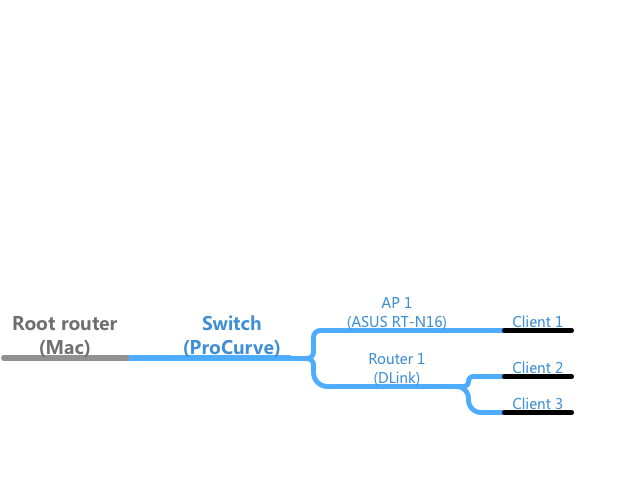
\includegraphics[width=\textwidth]{images/Showcase-topology}
	\caption{Device topology of showcase}
\end{figure}

\subsection{Pre-configuration}

\subsubsection{Configure the MAC address of the network devices}
The network devices could be Router, Switch or AP(access point). Their addresses must be stored in a \textit{json} file.

\paragraph{devices.json} stores the devices information as well as the topology map of the network. To configure the topology map, the device's name and all the MAC address are needed.

A sample is listed below:

\begin{lstlisting}[language=json,firstnumber=1,caption={Code segments of \textit{devices.json}}]
{
	"interfaces": [
	{
		"mac": "D2:00:1D:59:C3:E0",
		"media_index": 8,
		"name": "en2",
		"status": "active",	
		"link": "00:1C:2E:0E:AA:3F",
	},
	],
	"name": "Jin-Mac",
	"position": "Unknown",
	"snmp": 2,
	"status": true,
	"type": "router"
},

{
	"interfaces": [
	{
		"mac": "BC:EE:7B:97:41:2C",
		"media_index": 5,
		"name": "en0",
		"status": "active"
	}
	],
	"name": "ASUS",
	"position": "Asus-company",
	"snmp": 0,
	"status": true,
	"type": "ap"
},

{
	"interfaces": [
	{
		"mac": "00:1C:2E:0E:AA:3F",
		"media_index": "1",
		"link": "BC:EE:7B:97:41:2C"
	},
	{
		"link": "BC:EE:7B:97:41:2C",
		"mac": "00:1C:2E:0E:AA:3E",
		"media_index": "2"
	}
	],
	"name": "ProCurve",
	"position": "Berlin",
	"snmp": 1,
	"status": true,
	"type": "switch"
}
\end{lstlisting}

This JSON file contains for now three devices: „Jin-Mac“ as router and the root server, „ProCurve“ as a switch and „ASUS“ as an AP.

The topology structure of the network devices are also have to be configured.
In this experiment, media interface 8 of \textit{Jin-Mac} connects to media interface 1 of \textit{ProCurve}, media interface 2 of \textit{ProCurve} connects to media interface 5 of \textit{ASUS}.

\paragraph{config.json}

The \textit{config.json} file should also be configured, it contains two important fields: \textit{Host IP} and \textit{Host name}. \textit{Host IP} and \textit{Host name} is the IP address and name of the first-hop device(root device) in the flooding algorithm.

\begin{lstlisting}[language=json,firstnumber=1,caption={Code sample of \textit{config.json}}]
{
	"Host IP": "127.0.0.1",
	"Host name": "Jin-Mac"
}
\end{lstlisting}

\subsection{Locating process}

\subsubsection{Convert MAC and IP string to integer}

In the algorithm should do a lot of MAC address and IP address comparison, but the string format of MAC and IP is not proper for comparison. For example, the MAC address has several formats: uppercase string (0:1C:2E:E:AA:0), lowercase string (0:1c:2e:e:aa:0), with leading zero ( 00:1c:2e:0e:aa:00) or without leading zero ( ), separated by colon(:) or minus(-). That's why it shall be converted to an integer.

The int type of Python is 64 digits, so it is enough to contain the 48 digits MAC address.

So the MAC and IP string will be converted to integer number, it will also faster the comparison.

\subsubsection{Generate MAC-device-dict}

\textit{"dict"} means \textit{dictionary}, is a key-value pair data structure of Python. It's like the HashMap class in Java.

The MAC-device-dict is a dict object, using MAC as the key and device as the value.

\subsubsection{Generate structure of network topology}

The devices are stored as list, but the actual network should be organized as a tree, that's why it shall be converted to another topology structure.

\subsubsection{Query}

On the server web page, only the IP address of the client could be fetched from the HTTP headers. The \textit{request} parameter of a Django view contains the IP address of the client.

When the client IP address is fetched, the \textit{ipNetToMedia} table should be queried using \textit{snmptable} command.

\begin{lstlisting}[language=bash, caption={List all connected devices}]
$ snmptable -v 2c -c public <Host IP> ipNetToMedia
\end{lstlisting}

A typical output listed below:

\begin{lstlisting}[numbers=left, firstnumber=1, numberfirstline=true]
ipNetToMediaIfIndex ipNetToMediaPhysAddress ipNetToMediaNetAddress ipNetToMediaType
5 4c:9:d4:4d:d0:d6 192.168.1.1 other
5 ff:ff:ff:ff:ff:ff 192.168.1.255 other
8 8c:bf:a6:a7:17:63 192.168.2.2 other
8 10:40:f3:9f:49:e2 192.168.2.5 other
8 0:1c:2e:e:aa:0 192.168.2.7 other
8 ff:ff:ff:ff:ff:ff 192.168.2.255 other
\end{lstlisting}

The forth row is the mobile phone that we want to find out. In this row, number 8 indicates the media interface, \textit{8c:bf:a6:a7:17:63} and \textit{192.168.2.2} is the MAC address and IP address of the mobile phone.

Search the \textit{devices.json} file, media interface 8 connects to the ProCurve switch media interface 1.

And the ProCurve switch media interface belongs to ProCurve switch. This device is defined as a switch, supports SNMP 1, and is active.

The next device to be queried is the ProCurve switch, using command

\begin{lstlisting}[language=bash, caption={Query the ProCurve switch}]
$ snmpwalk -v 2c -c public 192.168.2.7 mib-2.17.7.1.2.2.1.2
\end{lstlisting}

It will output the demanded information, a sample is listed below:

\begin{lstlisting}
SNMPv2-SMI::mib-2.17.7.1.2.2.1.2.1.0.28.46.14.170.0 = INTEGER: 0
SNMPv2-SMI::mib-2.17.7.1.2.2.1.2.1.16.64.243.159.73.226 = INTEGER: 1
SNMPv2-SMI::mib-2.17.7.1.2.2.1.2.1.88.176.53.243.205.40 = INTEGER: 3
SNMPv2-SMI::mib-2.17.7.1.2.2.1.2.1.90.176.53.63.244.100 = INTEGER: 3
SNMPv2-SMI::mib-2.17.7.1.2.2.1.2.1.140.191.166.167.23.99 = INTEGER: 1
SNMPv2-SMI::mib-2.17.7.1.2.2.1.2.2.0.28.46.14.170.1 = INTEGER: 0
\end{lstlisting}

Care the fifth line, the value 140.191.166.167.23.99 is the decimal format of the MAC address, and it equals to 8c:bf:a6:a7:17:63. After the analyses of this line, it's known that the target mobile phone connects to the media interface 1 of the ProCurve switch.

Again, from the \textit{devices.json} configurations file, we know that the media interface 1 of the ProCurve switch connects to ASUS. The configuration shows that ASUS is an AP and it doesn't support SNMP, so it shall not have any sub device. So the ASUS router is returned as the device that directly connects to the mobile phone.
